\documentclass[border=10pt]{standalone}
\usepackage[svgnames]{xcolor}
\usepackage{amsmath}
\usepackage{pgfplots}
\pgfplotsset{compat=newest}
\usepackage[sfdefault]{FiraSans}
\usepackage{FiraMono}
\renewcommand*\familydefault{\sfdefault}
\begin{document}
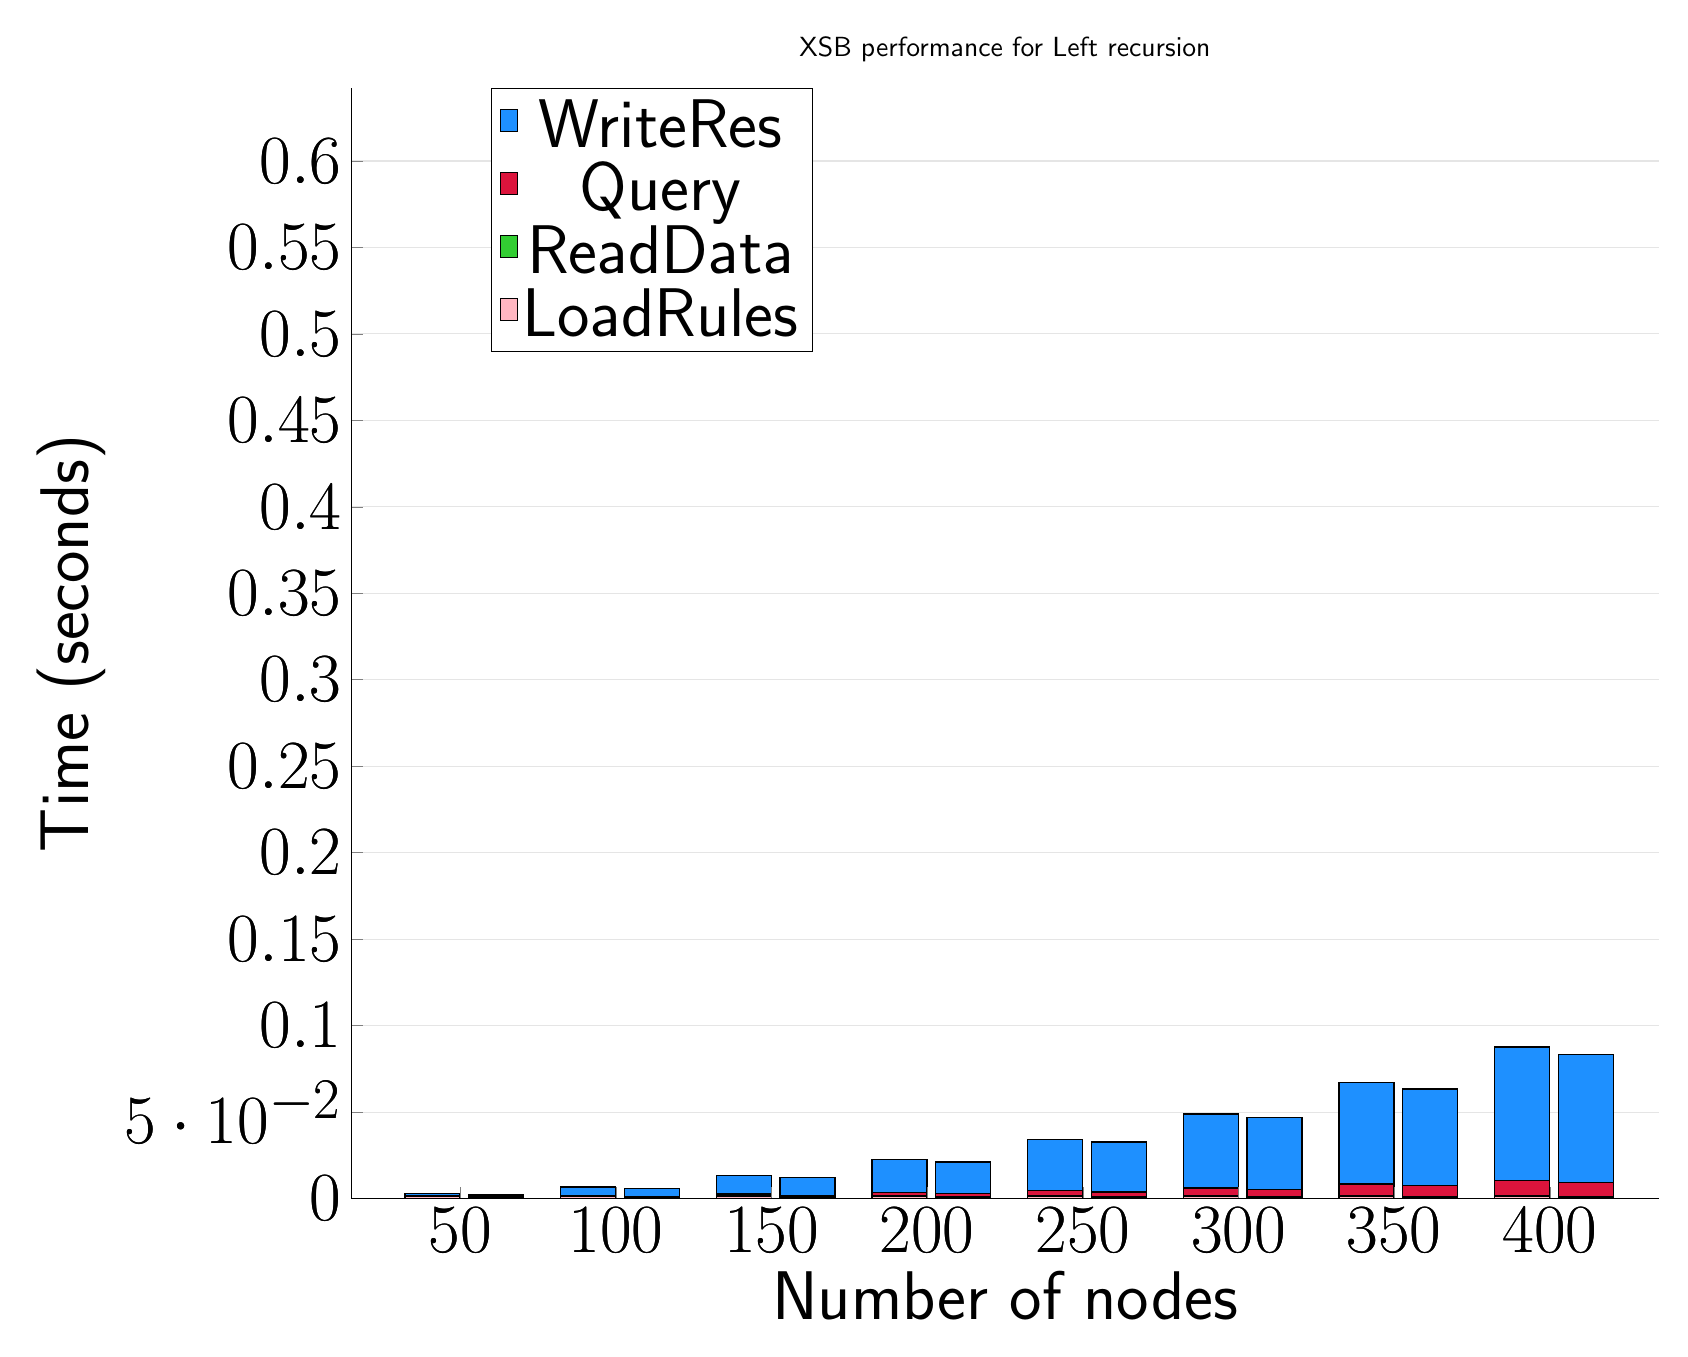
\begin{tikzpicture}
	\begin{axis}[
			ybar stacked,
			title={XSB performance for Left recursion},
			bar shift=-10pt,
			width=1.5\textwidth,
			bar width=0.7cm,
			ymajorgrids, tick align=inside,
			major grid style={draw=gray!20},
			xtick=data,
			ymin=0, ymax=0.6422704648971556,
			axis x line*=bottom,
			axis y line*=left,
			enlarge x limits=0.1,
			legend style={
					at={(0.23, 1)},
					anchor=north,
					legend columns=1,
					font=\Huge,
				},
			ylabel={Time (seconds)},
			xlabel={Number of nodes},
			label style={font=\Huge},
			tick label style={font=\Huge},
		]
		\addlegendimage{fill=DodgerBlue, draw=black, line width=0.2pt}
		\addlegendentry{WriteRes}
		\addlegendimage{fill=Crimson, draw=black, line width=0.2pt}
		\addlegendentry{Query}
		\addlegendimage{fill=LimeGreen, draw=black, line width=0.2pt}
		\addlegendentry{ReadData}
		\addlegendimage{fill=LightPink, draw=black, line width=0.2pt}
		\addlegendentry{LoadRules}
		\addplot +[fill=LightPink, draw=black, line width=0.5pt] coordinates {
				(50, 0.0010684013366699218)
				(100, 0.0010425806045532228)
				(150, 0.001047444343566894)
				(200, 0.0010660648345947271)
				(250, 0.001035928726196288)
				(300, 0.001062870025634767)
				(350, 0.001053595542907714)
				(400, 0.001057744026184082)
			};
		\addplot +[fill=LimeGreen, draw=black, line width=0.5pt] coordinates {
				(50, 0.0003624677658081056)
				(100, 0.0003997802734375)
				(150, 0.0004715681076049804)
				(200, 0.0005344629287719726)
				(250, 0.0005591630935668946)
				(300, 0.0006115913391113281)
				(350, 0.0006659269332885742)
				(400, 0.0007020950317382814)
			};
		\addplot +[fill=Crimson, draw=black, line width=0.5pt] coordinates {
				(50, 0.0001341581344604492)
				(100, 0.0005071401596069336)
				(150, 0.001119017601013185)
				(200, 0.001977872848510742)
				(250, 0.003100228309631348)
				(300, 0.004501533508300783)
				(350, 0.006615805625915526)
				(400, 0.008700299263000488)
			};
		\addplot +[fill=DodgerBlue, draw=black, line width=0.5pt] coordinates {
				(50, 0.0014129400253295888)
				(100, 0.0048330783843994135)
				(150, 0.010813784599304186)
				(200, 0.018955922126770015)
				(250, 0.029603528976440436)
				(300, 0.04282987117767334)
				(350, 0.05889017581939697)
				(400, 0.07712614536285403)
			};
	\end{axis}
	\begin{axis}[
			ybar stacked,
			bar shift=13pt,
			width=1.5\textwidth,
			bar width=0.7cm,
			ymajorgrids, tick align=inside,
			major grid style={draw=none},
			xtick=data,
			ymin=0, ymax=0.6422704648971556,
			axis x line*=none,
			axis y line*=none,
			enlarge x limits=0.1,
			label style={font=\Huge},
			tick label style={font=\Huge},
		]
		\addplot +[fill=LightPink, draw=black, line width=0.5pt] coordinates {
				(50, 0.0006029999999999999)
				(100, 0.0006035000000000003)
				(150, 0.0006086000000000005)
				(200, 0.0006151000000000002)
				(250, 0.0005991000000000003)
				(300, 0.0006162999999999996)
				(350, 0.0006131999999999998)
				(400, 0.0006004000000000001)
			};
		\addplot +[fill=LimeGreen, draw=black, line width=0.5pt] coordinates {
				(50, 0.0001740999999999999)
				(100, 0.000215)
				(150, 0.0002636999999999997)
				(200, 0.0003121000000000001)
				(250, 0.0003459999999999999)
				(300, 0.00039950000000000066)
				(350, 0.0004341999999999993)
				(400, 0.0004806999999999998)
			};
		\addplot +[fill=Crimson, draw=black, line width=0.5pt] coordinates {
				(50, 0.00012520000000000022)
				(100, 0.0004805000000000008)
				(150, 0.0010642999999999998)
				(200, 0.0018938)
				(250, 0.0029652000000000003)
				(300, 0.0042975999999999995)
				(350, 0.006340799999999999)
				(400, 0.008348499999999998)
			};
		\addplot +[fill=DodgerBlue, draw=black, line width=0.5pt] coordinates {
				(50, 0.0011692999999999999)
				(100, 0.004517799999999999)
				(150, 0.0103823)
				(200, 0.0184286)
				(250, 0.0288118)
				(300, 0.0414263)
				(350, 0.056022300000000004)
				(400, 0.0739252)
			};
	\end{axis}
\end{tikzpicture}

\end{document}
